\documentclass[12pt,a4paper]{article}

\usepackage[dvips]{graphicx}
\usepackage[dvips]{color}
\usepackage{amsbsy, marvosym}
\usepackage{amsmath}
\usepackage{paralist}
%\usepackage{algorithm2e}
\usepackage{algorithmic}
\usepackage{algorithm}
\usepackage{subfigure}
\usepackage{lscape}
\usepackage{booktabs}
\usepackage{lscape}
\usepackage{natbib}

\newcommand{\HRule}{\rule{\linewidth}{0.5mm}}

\pagestyle{plain}
\textwidth 16cm
\textheight 23cm
\oddsidemargin -0.5cm
\evensidemargin -0.5cm
\topmargin 0cm

\usepackage{float}
\floatstyle{ruled}

\newfloat{program}{thp}{lop}[section]
\floatname{program}{Program}

\newfloat{note}{thp}{lon}[section]
\floatname{note}{Note}

\begin{document}
\pagenumbering{arabic}
\setlength{\parindent}{5mm}
\setlength{\parskip}{10pt plus2mm minus2mm}
\thispagestyle{empty}



% TITLE

\begin{titlepage}
 
\begin{center}
 
% Upper part of the page
%\includegraphics[width=0.15\textwidth]{./logo}\\[1cm]
 
\textsc{\LARGE Liverpool John Moores University}\\[1.5cm]
 
\textsc{\Large Ph.D Transfer Report}\\[0.5cm]
 
 
% Title
\HRule \\[0.4cm]
{ \Large \bfseries Adaptive Optimal Telescope Scheduling}\\[0.4cm]
 
\HRule \\[1.5cm]
 
% Author and supervisor
\begin{minipage}{0.4\textwidth}
\begin{flushleft} \large
\emph{Author:}\\
Stephen \textsc{Fraser}
\end{flushleft}
\end{minipage}
\begin{minipage}{0.4\textwidth}
\begin{flushright} \large
\emph{Supervisor:} \\
Prof. Iain \textsc{Steele}
\end{flushright}
\end{minipage}
 
\vfill
 
% Bottom of the page
%{\large \today}

{\large November 19, 2009}

 
\end{center}
 
\end{titlepage}


\newpage
\tableofcontents

%\title{Adaptive Optimal Telescope Scheduling
%Ph.D Transfer Report}
%\author{S.N. Fraser}
%\date{\today}
%\maketitle

%-------------------------------------------
%
%-------------------------------------------
\newpage
\section{Introduction}

The Liverpool Telescope (LT) \citep{steele04lt} is a fully robotic 2 metre astronomical telescope situated at the Observatorio de los Roches de los Muchacos on La Palma in the Canary Islands. It operates without supervision, controlled by an integrated suite of software systems. The Robotic Control System (RCS) is responsible for deciding on the mode of operation and for protecting the telescope. It controls the telescope and its instruments and receives environmental information via a number of lower level subsystems. The Telescope Control System (TCS) is responsible for slewing the telescope axes onto targets and for tracking them through the night. The Instrument Control Systems (ICS) are responsible for configuration of the suite of scientific instruments, taking exposures, reading out, saving to disk and control of real-time data reduction pipelines (DPRT). The Observer Support System (OSS) comprises the scheduler and observing database (ODB) along with its access interface. The ODB contains all the information required to perform the observations - target locations, instrument selection and configuration, exposure times and options for autoguiding and acquisition. The RCS makes requests to this scheduler at various times for groups of observations to perform. These are then executed and results reported back.

\subsection{Context}

A  series of characteristics that can contribute to a \emph{good} schedule are defined in \citep{steele97control}. They mention fairness (of time allocations between various committees), efficiency (quality of observations, minimization of idle time) and feasibility (is the target visible, is the seeing good enough). 

The first version of the LT scheduler \citep{fraser04scheduling} is a simple despatch scheduler. A list of candidate observations is generated by checking requested timing and observing constraints against the current conditions. These observations are then scored using an objective function formed using a weighted sum of a set of metrics. The highest scoring observation is then selected for execution.

Proposals represent an astronomers observing program and collect together information required to perform the client's observations along with time and resource accounting. The unit of scheduling is termed a group and consists of the specifications of the exposures, timing requirements, sequencing, observing condition constraints and quality of service metrics. 

Each group has a set of enablement windows representing those intervals during which it \emph{should} be observed if possible - these are obtained from the group's timing constraints. 

The times when the group can \emph{actually} be observed are further constrained by a number of factors:-
\begin{itemize}
\item Observations are only performed at night - in some cases we further restrict this to the period between evening and morning astronomical twilight.

\item Environmental constraints, some of which are deterministic e.g. only observe this target if the moon is greater than distance \emph{x} away from the target or only observe if the target is above elevation \emph{y}. Others are less predictable, e.g. only observe this target if the atmospheric seeing is less than \emph{z} arc seconds. 

\item Observations cannot be made during bad weather (the dome is closed to protect the instruments) and there is no point observing in cloudy conditions.

\item There are unpredictable target-of-opportunity interrupts where external intelligent agents \citep{guidorzi06automatic, tsapras09robonet} may take over the telescope for a period with no advance warning.

\item There are certain periods, sometimes known in advance, when the telescope is unavailable due to engineering or local or remote manual observing.

\end{itemize}
 
These factors taken together make long-term planning difficult, and were the primary reason for initially developing a despatch scheduler.

\subsection{Aims and objectives}

The primary aims of this project are to investigate the fundamental components required to develop a software framework with which a range of observatory schedulers can be built and to test the effectiveness of a variety of schedulers so built against real and artificial problem and environmental scenarios using a suitable set of quality metrics. 


\subsubsection{Objectives for M.Phil}

\begin{enumerate}
\item Investigate metrics with which to compare the efficiency and quality of generated schedules.

\item Design software instrumentation to embed within the current robotic control system to collect data with which to characterize the operating environment.

\item Using data collected by the embedded software, I will design a simulation framework incorporating knowledge of the operating environment and ODB characteristics with which to test any schedulers developed.

\item Develop a despatch scheduler as a baseline with which to test more advanced schedulers, this will be capable of configuration to use different scheduling policies.

\item Tune the baseline scheduler using various controllable parameters, typically objective weighting functions and bias function, to investigate the limits of this scheduling paradigm in the telescope scheduling context.
\end{enumerate}

\subsubsection{Additonal objectives for extension to Ph.D}

\begin{enumerate}
\item I will develop a look-ahead scheduler incorporating short-term prediction of environmental statistics to allow advanced planning of observations with a view to improving efficiency/gain.

\item Investigate variation of scheduling control parameters and horizon length on quality of schedules generated under varying environmental models to determine how to adapt to these - the quality of schedules generated will be compared to those generated by the baseline system.

\item Knowledge gained from this investigation will be incorporated into a final adaptive, look-ahead scheduler.

\end{enumerate}

%-------------------------------------------
% REVIEW
%-------------------------------------------
\newpage
\section{Literature Review}

There is a vast literature on the subject of scheduling covering both generic problems and highly domain-specific problem areas. In this section I present a brief introduction to some general techniques and review a number of specific case-studies. The constructive and iterative schedule building paradigms are introduced in section~\ref{subsect:constructive} and section~\ref{subsect:iterative} respectively. Section~\ref{subsect:search} details a number of search techniques used to speed up the scheduling process. A number of individual case studies are described in section~\ref{subsect:casestudy}. Flexible scheduling methods are detailed in section~\ref{subsect:flexible}. Section~\ref{subsect:reactive} provides examples of reactive scheduling systems. The use of artificial intelligence (AI) techniques including adaptive methods are described in section~\ref{subsect:adaptive} 

\subsection{Constructive techniques}
\label{subsect:constructive}
The constructive approach to generating schedules starts from an empty schedule and progressivly selects tasks to assign to time slots, gradually building up a schedule - effectively a path through the search space. As the search progresses deadend points may be reached when a task becomes unassignable - the search must then backtrack, unwinding previous assignments and attempting to reassign tasks in order to avoid the deadend. An uninformed search can be very inefficient, however search performance can be improved by using domain knowledge (heuristics) via some of the following techniques:- \footnote{In this context, \emph{variable} refers to some resource which is to be allocated - often this is just \emph{time}}

\begin{description}
\item[Variable ordering heuristics]
determine the order in which variables are selected for assignment - e.g. select the task for assignment that leaves the most options left for remaining task.A number of variable ordering heuristics used in the MicroBOSS scheduler are described in \citep{sadeh91lookahead}. The \emph{MinimumWidth} heuristic selects the variable with the fewest arcs i.e. constraint associations with other variables. Their \emph{operation resource reliance} (ORR) heuristic selects the task which relies most on the most contended resource or time period. The \emph{minconflicts} heuristic \citep{minton92minconflicts} selects a variable that is in conflict and adjusts its value until it is no longer in conflict.

\item[Value order heuristics]
determine how the value is chosen to assign to a selected variable. A \emph{filtered survivable schedules} (FSS) heuristic described in \citep{sadeh91lookahead} assigns to an operation the time-slot which is likely to be compatible with the largest number of survivable schedules = chance of surviving competition with other operations for possession of a resource (time).

\item[Constraint propagation]
allows more general improvements to be made. The implications of a constraint on a variable are tested against the constraints on other connected variables. Conflict analysis though costly (typically $O(e^n)$) \citep{muscettola92bottleneck} can reduce backtracking by pruning the search tree. There is a trade-off in the time taken to perform the consistency checking and the reduction in problem size generated. In \citep{johnston94spike} the use of node , arc and path consistency is used to prune the search space for scheduling observations with the Hubble Space Telescope (HST). 

\item[Deadend recovery heuristics] 
The occurance of deadends resulting in the need to perform backtracking indicates that the chosen variable and value ordering heuristics and consistency enforcing technique are insufficent to cope with the problem in hand, a consequence of re-application of these same heuristics on backtracking is that the same deadends may be encountered repeatedly - a thrashing effect similar to that which occurs sometimes in disc access. Recovery heuristics are designed to allow for more intelligent choice on how to backtrack. Several general techniques for improving backtracking search are described in \citep{sadeh94backtracking}. These use the \emph{partial conflict set} of the deadend (i.e. the set of activities which have blocked progress of the search at that point and which may have been involved in previous deadends). Their \emph{Incomplete Backjumping Heuristic} (IBH) uses texture based measures \citep{beck97texturebased} to identify assignments which are estimated to lead to more global solutions then when a deadend is detected unwinds to this critical assignment and tries alternatives.

\end{description}



%
% Iterative Repair techniques
%
\subsection{Iterative repair}
\label{subsect:iterative}
The iterative repair technique starts by generating a complete but not neccessarily optimal or even valid schedule. Retraction heuristics are used to remove conflicting or oversubscribed tasks or resources. Repair heuristics are then used to re-insert task(s) at appropriate places. Repair may occur as part of a search process to find an optimal schedule from a preliminary first guess, or may be used in a reactive context to fix an already executing schedule disrupted by unexpected changes to the environment or goals or used opportunistically to take advantage of such changes to increase the global value. An iterative repair system for spacecraft mission planning is described in \citep{rabideau99iterative}.

\subsection{Search techniques}
\label{subsect:search}
Whether generated by a constructive or repair technique, scheduling is invariably a search process. Mechanisms for speeding up search have been an active areas of research for some time.

\begin{description}
\item[Local search]
Greedy search, also known as hill-climbing or gradient descent is the classic technique. The search proceeds by moving step-by-step up the locally steepest gradient to the peak (of the objective function). This type of search can become trapped at local maxima, there is no means of escape to allow the search to explore other parts of the space.

\item[Search with noise]
In an attempt to escape local maxima a number of techniques have been developed to allow a degree of random movement around the search space. Such a system \emph{Heuristic-biased stochastic sampling}, described in \citep{bresina96hbss} which uses heuristic knowledge to bias the direction of search is used to improve the speed of searching for optimal schedules for the Fairborne Observatory. This approach is extended in \citep{cicirello02amplification} and \citep{kramer04swapping} who consider a number of different randomization techniques. 

\item[Simulated annealing]
Based on an analogy to the cooling of molten materials, simulated annealing is a technique which allows a search to make random jumps around the solution space to discourage the search becoming trapped in local minima. The size and likelihood of the jumps decreases as the search progresses towards convergence by lowering the annealing temperature. This technique is used to effect in the GERRY system \citep{zweben94scheduling} for space shuttle ground operations.

\item[Adaptive noise]
This technique is introduced in \citep{hoos02adaptive} for a series of general search problems, but basically allows the degree of randomization to adapt to the rate of convergence. This technique is applied to the scheduling of spacecraft operations in the ASPEN system \citep{fukunaga04robust} .

\item[Moving search]
Similar to a predator-prey scenario - catching a moving target. A technique is described in \citep{yokoo99search} for situations where the goals change as the search proceeds.


\item[AMP]
Adaptive Memory Programming \citep{taillard98adaptive} was first coined as a general term for a class of optimization techniques which use some form of memory to retain knowledge about poor parts of the search space which have been visited recently.

In TABU search \citep{glover99tabu}, as the space around a solution is searched the memory keeps track of bad directions and avoids entering these \emph{taboo} areas. Such a system \emph{Squeaky Wheel Optimization} is described in \citep{joslin99squeaky} .  

In scatter search new solutions are generated by evolving existing solutions in a process similar to that used in Gentic Algorithms in that parts of \emph{fit} solutions are combined to yield new solutions which may be expected to retain some of the \emph{fitness} of the parents. 

\end{description}

\subsection{Case studies}
\label{subsect:casestudy}
%\subsection{Partially Ordered Schedules (POS)}
Conflict Partition scheduling (CPS) is described in \citep{muscettola92bottleneck} for solving scheduling problems by identifying regions of the search space where bottleneck conflicts occur and posting constraints to move the search away from these regions where solutions are unlikely to be found. Bottlenecks are identified as those points where the most resource contention occurs and additional sequencing constraints are posted to reduce the contention. 
%They employ two measures of contention - \emph{token demand} $\Delta(\tau,t_i)$ measures how much a token or task $\tau$ relies on a time slot $t_i$ by counting the number of simulations in which $\tau$ was asssigned to $t_i$, \emph{resource contention} $X(\rho,t_j)$ measures how many tokens are competing for a resource $\rho$ at time $t_j$ by counting the number of simulations in which $\rho$ is requested during $t_j$.

The GERRY system for scheduling space shuttle ground operations is described in \citep{zweben94scheduling} . They define 3 types of constraint:- \begin{inparaenum}[(\itshape a\upshape )] \item temporal constraints represent precedences between activities, \item resource constraints represent usage of resources and \item state constraints represent particular environmental state variable assignments required by some activities - certain activities, denoted as \emph{achievers} are able to set these variables \end{inparaenum}. A weighted penalty function is used to measure the cost of constraint violation. Their repair procedure considers each type of constraint seperately and handles repair of $N$ of each type per cycle before moving onto the next cycle. In order to avoid trapping at local optima in the search space they employ simulated annealing to determine acceptance of a newly generated schedule. %At each iteration the cost of the current schedule $s$ is compared to the best so far $s^*$ and is accepted with a probability $P(s,s^*) = \exp{-\frac{|cost(s)-cost(s^*)|}{T}}$ where $T$ is the \emph{annealing temperature} which is cooled during the search. To resolve resource constraints tasks are selected for repair using 3 heuristic criteria \begin{inparaenum}[(\itshape i\upshape )] \item \emph{fitness} - move the task whose resource requirements match the amount of over-allocation most closely - the logic here is that a task which has a small resource requirement is less likely to have much effect, one which has a very large requirement will cause problems wherever it gets moved to, \item \emph{dependency} - move the task which has the fewest temporal dependants - a task with a large number of dependencies will likely cause additional violations when it is moved and disrupt existing assignments, \item \emph{distance} - move the task which needs the smallest move to resolve the conflict - a large move is likely to perturb the overall schedule more. \end{inparaenum}. The results of these metrics are scored and a task selected for the move. State constraints are repaired using a selection of 5 methods in priority order which involve moving the affected task and/or adding \emph{achiever} tasks into the schedule before the affected task to set the variable appropriately. 
The GERRY scheduler was found to be very effective in the chosen domain and was incorporated into the NASA Ground Processing Scheduling System (GPSS) an interactive tool for scheduling repair and refurbishment of the space shuttles between missions. 

The OPortunistic Intelligent Scheduler (OPIS) system is described in \citep{smith95reactive}. This introduces multi-perspective scheduling in which a number of complimentary schedule repair techniques are employed under the supervision of a Top Level Manager (TLM) and working through a common blackboard representation of the current solution and constraints. External events (changes to requirements, feedback from execution) are fed into the blackboard via model update agents. Conflict classes are defined relative to a number of conflict metrics including:- conflict duration, conflict size, resource idle time, upstream slack, projected lateness. A number of agents analyse the conflicts which are then matched to fuzzy behavioural profiles. Schedule repair agents are then selected to apply an appropriate repair heuristic suited to the character of the conflicts. In the trade-off between opportunistic improvement and non-disruption to the current baseline, OPIS is biased towards the later though this is a function of the analysis and repair heuristics chosen. 

Subsequent work on DITOPS \citep{smith96mixed} an air transport scheduler led to the extension of OPIS into a pluggable object oriented framework OZONE (Object Oriented OPIS = $O^3$). This has since been used to implement a number of scheduling systems. .
%\subsection{AMC BarrelMaster} 
For scheduling inflight refueling and transport missions the AMC BarrelMaster scheduler \citep{smith04continuous} was developed using OZONE. In its normal mode of operation the scheduler has to assign times to new missions into an already built schedule. 

The mission requirements generally lead to heavy over-subscription of resources so various relaxation regimes can be considered.%:- over-allocation of 'reserved' resources, allowable delays, mission combinations, priority pre-emption (bumping). These are handled by selection of different pluggable combinations of these procedures. e.g. $Eval_{criterion}$ has implementations $Eval_{MinTardiness}$ $Eval_{MinFlyingTime}$ and $Eval_{MinOverAllocation}$, similarly there are several versions of $Gen_{Resources}$ and $Gen_{Intervals}$. A procedure \texttt{CombineMissions} allows pairs of missions to be combined to attempt a reduction in resource usage, this can be applied recursively to maximize the reduction in overall flying time required. 
 The primary goal of the AMC Allocator is to assign the most high priority missions, often lower priority missions will be left out even though some assigned high priority missions with greater flexibility are included - an incremental optimization procedure \texttt{MissionSwap} can be applied to try and insert unassigned low priority missions into the schedule by retracting existing commitments and re-assigning to free up slots. 

%\citep{kramer03maxflex} describe 3 heuristics which can be used to select the tasks for retraction:- \begin{inparaenum}[(\itshape a\upshape)] \item $MaxFlex$ - measures the ratio of required time to available time summed over all resources required by a mission and is an indicator of the flexibility of the mission, \item $MinConflicts$ (\citep{minton92minconflicts}) - measures the number of resource conflicts over a mission's execution interval, \item $MinContention$ - defined as $\frac {\sum_{C \in Conflicts_i} dur_C}{\sum_{r \in R_i ReqInt_{r,i}}}$ where $dur_C$ is the duration of conflict $C$ and $ReqInt_i$ is the required executon interval for mission $i$ measures the proportion of a mission's required interval that is in conflict. \end{inparaenum}. In \citep{kramer04swapping} they extend this technique to minimize disruption to the existing schedule and to speed up the process by search tree pruning. (task pruning - interval pruning - depth bounded search / biased stochastic retraction - VBSS = ACO  - defer to that section or see.section~ XXX?)...

Work by NASA JPL on the ASPEN scheduling framework is described \citep{rabideau99iterative}. This is a constraint based search/optimization system intended for spacecraft operations scheduling. During the constraint satisfaction cycle, activities are slotted into the schedule and conflicts detected. The system then classifies these conflicts into a large set depending on the type of constraint broken or the type of resource bottleneck. A prioritized sequence of repair heuristics is then selected in turn to attempt a repair which moves closer to satisfycing.

 %ASPEN allows the specification of a number of search heuristics to be slotted in at decision points in the algorithm - some generic ones are described \begin{inparaenum}[(\itshape i\upshape)] \item conflict sorting heuristic (a variable order heuristic)- prefers to repair conflicts which require adding new activities, \item repair selection heuristic - prefers to move an activity then adding activities then deleting activities, \item interval selection heuristic for activities being created or moved (a value order heuristic)- prefers intervals which do not create new conflicts then intervals which minimize new conflicts. \end{inparaenum}.

They move on to describe an extension to ASPEN \citep{rabideau00generic} to allow interleaved repair and optimization using \emph{experts} - these are software components implementing heuristic operations \emph{an expert is a link between changes in the plan and the change in quality}. A number of classes of user preferences are defined, some acting on a local level, others globally. These specify a mapping from local variables to scoring metrics - an example given is of a preference on the start time of one activity relative to the preceding one centred on a \emph{preferred} time gap and decreasing monotonically either side within cutoff limits.

\subsection{Contingency and flexibility methods}
\label{subsect:flexible}
%What can go wrong - new tasks arrive, resources fail (e.g. instruments offline),

%Motivation - localize changes, make them small, continuity of \emph{global plan}, reactive repair must be fast. 

%Approaches - contingency - build multiple futures, execution branches to cope with what might happen. 

%Different approaches \citep{policella03flexible} classifies these as:-

%\begin{description}
%\item[Robust solution] create a robust schedule with built in flexibility (time slop).
%\item[Partially defined schedules] Define partial order of activities.
%\item[Rescheduling] as already discussed.
%\item[Dynamic] Despatch scheduling.
%\end{description}

Three pro-active techniques for building extra time into a schedule to cope with uncertain duration are described in \citep{davenport01slack}. \emph{Temporal protection} adds a slack time into each activity duration prior to the search, \emph{time slack window} uses reasoning during the search to attach minimum slack into each activity, \emph{focused time window slack} (FTWS) assigns slack based on the distance along the planning horizon. Normal distributions  are used to model the likelihood (MTBF) $N(\mu_{tbf}, \sigma_{tbf})$ and length (downtime) $N(\mu_{dt}, \sigma_{dt})$ of breakdowns:-
When tested on simulated problems with varying degrees of uncertainty (breakdowns) all methods help improve tardiness with increasing degrees of uncertainty. They do not however give account of the tradeoff due to uneccessary slack time introduced by the technique relative to the gains of continuity and reduced need for rescheduling.

Two different approaches are compared \citep{policella03flexible} and described in more detail \citep{policella05thesis}. 
They define 3 measures of robustness - \begin{inparaenum}[(\itshape a\upshape )]\item reactiveness - speed of response, \item stability - degree of change induced by reaction - ripple effect, \item solution quality - preservation (or enhancement) of performance relative to baseline schedule.\end{inparaenum}.

The first technique \emph{resource envelope based} employs a 2 step process. 
In the first step, from an initial partially ordered schedule with constraints they compute the resource-envelope (a time varying measure of resource requirements), using this they then detect conflicts (where more activities require a resource than its capacity allows), a selection heuristic is used to rank and then select a pair of competing activities, a sequencing heuristic then specifies (posts) new precedence constraints to remove this conflict. The resulting modified schedule with new constraints is fed back into the first step until a solution is found.
The second technique \emph{earliest start time} starts with a pre-selected fixed-time schedule, then selecting activities based on ranked order of start times and using a cheaper resource analysis posts new precedence constraints which can be used to determine the bounds for each activity to prodcuce a flexible schedule. They find that the second approach perfoms best against all quality measures and is fastest.  

A different approach is taken in \citep{bresina94jic}. Just-in-case (JIC) scheduling is applied to the selection of observations for the Fairborne Observatory in which the main source of uncertainty relates to the lengths of observations (action duration uncertainty). They run multiple simulations over the night looking for the most likely break points then look for alternative branches to execute. Later work \citep{bresina99increased} for Mars rover operations extended JIC to include resource uncertainty in addition to time uncertainty. They use an expected utility measure to select branches rather than just failure probability and allow setup steps prior to branch points.

\subsection{Reactive scheduling}
\label{subsect:reactive}
Deals with the repair of executing schedules which have become inconsistant or broken due to changes in the environment. If the goals (objectives) are changed dynamically, an executing schedule may break or become sub-optimal, reactive scheduling deals with this situation also. A subclass of reactive scheduling is dynamic scheduling, where the decision of what to schedule next is made at that point in time - there is no look-ahead though the history of the execution to date may be available.

Two classes of reactive system are described in \citep{jones98survey}:-
\begin{itemize}
\item reactive repair - the system waits for an event to occur before attempting to recover the system.
\item in pro-active adjustment the system monitors continuously, predicting the future evolution and attempting to plan ahead for contingencies while the plan is executing.
\end{itemize}

\subsection{Adaptive Learning techniques applied to scheduling}
\label{subsect:adaptive}
In dynamic systems \citep{shaw90intelligent} it is hypothesised that the rules used to make scheduling decisions should change with time as the problem characteristics evolve. They proposed a system which distinguishes between and ranks problem characteristics by relative importance, then performs adaptive scheduling by opportunistically selecting appropriate heuristics in a system called Pattern Directed Scheduling (PDS)
% works in 2 stages. In the first step (learning stage) a series of training scenarios are simulated and used to study the effects of applying various despatching rules. A critic module (the expert) analyses the performance of these rules on the problem scenarios and may generate new training examples to refine the matching of patterns to rules. The system chosen for induction was based on Iterative Dichotomizer 3 ID3 \citep{quinlan86induction}, in this system a tree of rules is built up by splitting the domains of the problem attributes (summary explanation in Hopgood KBS for E and S). 

Case based reasoning (CBR) is a learning technique in which rules are induced by matching problem situations against a set of examples (the cases). CBR is particularly useful at extracting rules from noisy data. It operates incrementally building up its knowledge base while working so there is no large expenditure of effort at the start of the process or any need to check consistency between rules as in a rule-based learning. Contextual information may be retained in the cases to help human assessors to understand the induced rules.

Due to their interactions and conflicts, it is often difficult to determine numerically or in terms of hard-and-fast rules, the relative ranking and trade-offs between users' schedule optimization preferences. The CABINS system \citep{miyashita95cabins} uses CBR to capture these preferences. CABINS provides a framework for acquiring preferences then uses the case base to improve schedules and provide a reactive repair mechanism in response to unforseen events. 

The CABINS framework is extended \citep{sycara96case} to consider time-varying user preferences. Their extension allowed the system to learn new cases from its own evaluations of schedule improvment while running. They employed a \emph{rolling horizon} model in which the matching algorithm gives more weight to recent cases than to older cases.


%-------------------------------------------
% WHAT WAS DONE
%-------------------------------------------
\newpage
\section{Work to date}

In section~\ref{subsect:metric} I describe a number of metrics used to characterize and measure performance of schedulers. In section~\ref{subsect:ecs} I provide details of a study of the weather and atmospheric environment at the telescope site relevant to scheduling. Section~\ref{subsect:sca} provides a brief summary of the software component architecture (SCA) the design of which is a major outcome of the overall project. A basic despatch scheduler built using SCA is described in section~\ref{subsect:bds} along with details of some shakedown experiments. The work in the remaining sections consists of additional work beyond the original plan for M.Phil. In section~\ref{subsect:mam} I describe a man-against-machine study used to provide a comparison and baseline. Finally in section~\ref{subsect:lts} I describe in more detail a long period study designed to examine the behaviour of 2 types of scheduler in varying environmental conditions.

\subsection{Metrics study}
\label{subsect:metric}
Metrics are quantative standards for measuring performance, quality or some aspect of a service or process we wish to monitor. In the context of scheduling these can be broadly divided into problem complexity metrics and schedule quality metrics.

\begin{description}
\item[Problem complexity metrics (PCM)] measure the difficulty of a scheduling problem and provide an independant variable with which to asses the performance of schedulers. The following metrics have been investigated:-

\begin{itemize} 
\item Contention profile $C_c$ is the time evolving profile of the number of observation groups which \emph{could} be scheduled according to their explicit timing constraints. The average contention over the course of a night gives an estimate of how overloaded the schedule could potentially be.

\item Demand $C_d$ is defined as the sum of the ratio of \emph{expected execution time} to \emph{length of available execution window} for all those groups which are enabled at a given time. If this aggregate demand exceeds unity then it is likely that some of the groups will not be observed i.e. the requirement for time is greater than the time available

\item Load $C_L$ is a fairly simple metric which describes the ratio of total executable time in a given observing night to the length of the night (or astronomical night).

\end{itemize}
\item[Schedule quality metrics (SQM)] measure the actual performance of schedulers on problems characterized by PCMs. A number of potential  metrics have been devised including:-

\begin{itemize}

\item Optimal Height metric $Q_{OH}$ measures how close to the \emph{optimum} height the group is observed during its execution window. 

\item Priority metric $Q_{PX}$ measures the total priority score achieved i.e just sums up the priorities of the groups selected weighted by the amount of time spent performing the group on the basis that e.g. an hour of high priority is better than 2 lots of 10 minutes preforming low priority groups. 

\item Target demand metric $Q_{TD}$ measures how \emph{urgent} the selected groups are with reference to the night's demand profile $C_d$.
\begin{equation}
Q_{TD} = \frac{1}{L(S)}\sum_{g \in S}{f_D(g,t)}
\end{equation}
where $f_D(g,t)$ represents the value of the demand heuristic for group $g$ at execution instant $t$.

\item Execution target metric $Q_{XT}$ is a measure of the amount of the night during which groups are actively being observed. A low value is effectively an indication of \emph{slack time}.
\begin{equation}
Q_{XT} = \sum_{g \in S}{X(g,t)}
\end{equation}
where $X(g,t$) is the estimated execution time for group $g$ at execution instant $t$.

\item Remaining nights metric $Q_{RN}$ counts a decreasing function (for convenience 1/n) of the \emph{number of nights remaining} $n$ for any groups in the observability window $\Phi(g,t)$ at the time of selection/execution. It effectively measures how \emph{urgent} the current window is in terms of the number of future chances of being executed.
\begin{equation}
Q_{RN} = \sum_{g \in S}{\frac{1}{R(g,t,\Phi(g,t))}}
\end{equation}
where $R(g,t,\phi)$ counts the number of remaining nights for a feasiblity window $\phi(g,t)$ of group $g$ at execution instant $t$ - i.e. it counts the number of feasible sub-intervals of $\Phi$ with maximum of 1 per night.

\end{itemize}

\end{description}

\subsection{Environment characterization study}
\label{subsect:ecs}
An analysis of the environmental conditions at the telescope site has been performed in order to determine its characteristics and whether it would be feasible to make predictive assessments of future conditions (with a view to look-ahead scheduling).

Meteorological data has been collected on the ORM site for many years, in particular the largest and most comprehensive set of continuous meteorological station readings going back to 1985 have been recorded by the Isaac Newton Group (ING). Other telescopes on the site have meteorological data covering lesser periods. 

The ING annual report 2000-2001 \citep{ing00annual} gives details of weather downtime for the ING telescopes of around 20\% per year. The data for period 1991-2001 shows a variation between a minimum of 16\% annual loss in 1998 to a maximum of 37\% in 1996. Seasonally the minimum downtime of around 3\% occurs in summer (June,July,August) with increasing levels of downtime either side reaching a maximum of upto 40-45\% during the worst months of December and January. The 2005 annual report shows a peak of around 80\% weather loss during february 2005, a period during which the site was covered in snow for several weeks and observing was effectively prevented.

The atmospheric seeing regime has been studied for many years both through short campaigns and as part of longer studies aimed at site testing for telescopes such as the Grande Telescopio Canarias (GTC).
 A short study \citep{vernin92optical} on the contributions of the various air layers above the site suggests that the main contribution, some 50\% comes from air in the boundary layer (from a few meters to 1 km above the ground. They found that 40\% is provided by the free air above 1 km and that 8\% comes from the surface layer of the first few meters. Sources internal to the dome provide the remaining 2\%.

A longer 9 month study \citep{munoz97nighttime} using a DIMM mounted on a 5m tower (above the surface layer) concluded that the inversion layer which lies below the observatory site is of particular importance in determining seeing characteristics. %The layer generally lies between 1200m and 1500m, well below the site at 2400m and acts to suppress convection - a layer of strato-cumulus is generally seen at the top of this layer. Around 55\% of the local atmospheric humidity is trapped below the layer with around 20\% above. They find that the best seen correlates with those time when the inversion layer is at its lowest (around 1200m and strongest (largest temperature difference between top and bottom of the layer) which occurs in the summer months (June,July, August). At this time the strength of the trade winds is highest. 
They find that during the summer the average seeing is 0.61'' and median 0.5''. During the remaining months the average seeing is 0.77'' and median 0.91''. 

They also studied \citep{munoz97nighttime} some time variation effects finding that typically seeing can change very abruptly - deteriorating within a few minutes but that it rarely returns to a stable level so quickly - typically they find a recovery time of around 2 hours - they put this down to the effects of sudden perturbations in a steady atmospheric flow giving rise to turbulence which can take some time to settle. %Some oscillatory effects were recorded with a period of around 45 minutes. 

%A year long study by \citep{munoz98homogeneity} on the variation of seeing between different sites at the ORM revealed an average seeing of 0.72'' and median 0.65''. They found relatively small variation between sites except when the seeing was particularly poor when the variation was more pronounced - upto 0.2'' between locations. In summer they find that seeing is better than 0.5'' for 50\% of the time dropping to 25\% averaged over the whole year. A correlation was found between wind speed and direction and seeing quality. 

A study of the contributions to extinction at the ORM \citep{lapalma31}was made in 1985. This gives formulae for the calculation of the contributions from rayleigh scattering and absorption by ozone and water-vapor. They find that the contribution from ozone can vary significantly during the year and even on timescales of a few hours.

Weather data from the LT  has been obtained from 2 independant sources.
\begin{itemize}
\item Embedded software has been written to collect data from the LT's own weather monitoring system (WMS). This data has been collected for a period of 20 months/583 days at a cadence of approximately once every 32 seconds with very few gaps giving a total of 1582518 samples.
\item Observer reports of weather downtime hours per night (collated next day) for reporting on the telescope website. This data is bundled in with the technical downtime statistics and overrides these when both occur on the same night.
\end{itemize}

An investigation has been performed looking specifically at humidity data which has generally been found to be the deciding factor in weather shutdowns.

The distribution of humidity shown in Fig.~\ref{fig:met_humidity_dist} shows an approximately normal profile with a peak around 15\% and average of 40\%. A very sharp secondary peak occurs around 95-100\% humidity. With the RCS weather closure trigger levels set to 70\% (\emph{clear}) and 80\% (\emph{alert}), both can be seen to be well into the tail of the distribution just before the spike. This suggests that few false alerts should occur.

\begin{figure}[htbp]
  \begin{center}
    \includegraphics[scale=0.4, angle=-90]{figures/ecs/hum.dat.eps}
  \end{center}
  \caption[Relative distribution of humidity at telescope site.]
{Distribution of atmospheric humidity at the telescope site over all samples. The distribution shows a normal profile with peak around 15\% and average of \%. A very sharp secondary peak occurs around 95-100\% humidity. With the variable trigger levels set to 70\% good and 80\% bad these are in the tail of the normal distribution just before the spike level.}
  \label{fig:met_humidity_dist}
\end{figure}

A simple model for weather state prediction has been tested to determine if it might provide usable results.
The model is based on the assumption that the weather will continue in its current state for a period roughly equal to the length of time it has already been in that state continuously, thereafter the probability of maintaining this state decreases, assumed exponentially with a decay length some scaled fraction $m_{\tau}$ of the current stability period. Fig.~\ref{fig:good_bad_hum_dist} shows the variation of lengths of consecutive periods of good and bad weather based on humidity threshold (80\% trigger) and clearing stability time of 30 minutes. We see that shorter periods are most common with the average length of \emph{good} periods being 31.5 hours and bad periods being 7.7 hours. The overall fraction of time classified as \emph{good} resulted in 80.35\% of all time with \emph{bad} weather making up the remainder.

\begin{figure}[htbp] 
\begin{center}
    \includegraphics[scale=0.4, angle=-90]{figures/ecs/good_bad_hum_bin.eps}
\end{center}
\caption[Cumulative probability of lengths of good/bad weather runs.]
{Cumulative probability of lengths of good/bad weather runs.}
\label{fig:good_bad_hum_dist}
\end{figure}

A series of simulations were run using the extracted period data (Fig. {\ref{fig:good_bad_period_time}) to determine the effectiveness of this prediction mechanism. Every 15 minutes through the available period a determination is made of the current weather state and how long ($\tau_G$ \emph{good}) or ($\tau_B$ \emph{bad}) it has been in that state. A prediction is made for a number steps into the future (192 steps of 15 minutes constituting upto 48 hours look-ahead) using the rule specified in Eqn.\ref{eqn:prediction_decay}. At each step the prediction is compared to the actual weather state at the time and counted as either a hit (correct prediction) or miss (incorrect prediction). The final percentages are shown in Fig. \ref{fig:gbc_prediction} against look-ahead time for a number of decay scale factors $m_{\tau}$. The baseline of 80.35\% represents the worst we should be able to achieve on average based on long-term climatological prediction. Fig.~\ref{fig:gbc_m_crossover} shows the crossover point - the length of look-ahead where the prediction becomes worse than long-term climatological prediction as a function of the decay scale factor $m_{\tau}$. This is seen to converge towards a value of 30-31 hours which is close to the average length of \emph{good} weather period.

\begin{equation}
\label{eqn:prediction_decay}
P_{good}(\Delta T) = 
\begin{cases} 
\Delta T < \tau_G : & 1   \\ 
\Delta T > \tau_G, \tau_G < T_G : & e^{\frac{\Delta T-\tau_G}{m \tau_G}} \\
\Delta T > \tau_G , \tau_G > T_G : & e^{\frac{\Delta T-T_G}{m \tau_G-T_G}}
\end{cases}
\end{equation}


\begin{figure}[htbp]
\begin{center}
    \includegraphics[scale=0.4, angle=-90]{figures/ecs/gbc_period.eps}
\end{center}
\caption[Time variation of lengths of good/bad periods based on humidity level.]
{Time variation of lengths of good/bad periods based on humidity level.}
\label{fig:good_bad_period_time}
\end{figure}


\begin{figure}[htbp] 
  \begin{center}
    \includegraphics[scale=0.4, angle=-90]{figures/ecs/gbc_predict.eps}
  \end{center}
  \caption[Accuracy of look-ahead weather prediction using time decay model against look-ahead time]
  {Effect of time scaling-factor (m) on variation of prediction accuracy of time decay prediction model against look-ahead time. All plots show a decay with time. As the scale factor is increased the cross-over point for the prediction against climatological baseline prediction of 80.03\% approaches a maximum of around 31 hours. }
  \label{fig:gbc_prediction}
\end{figure}

\begin{figure}[htbp]
  \begin{center}
    \includegraphics[scale=0.4, angle=-90]{figures/ecs/m_crossover.eps}
  \end{center}   
  \caption[Variation of cross-over point for look-ahead weather prediction using time decay model with scale factor.]
  {Variation of cross-over point for look-ahead weather prediction using time decay model with scale factor. The crossover point is seen tn converge on a value around 30-31 hours which corresponds closely to the average length of good weather periods (31.5 hours).}
  \label{fig:gbc_m_crossover}
\end{figure}


Seeing, caused by micro-turbulence in the atmosphere affects observing by spreading the point source image out and limits resolution.

Embedded software has collected seeing data generated by the LT's instrument reduction pipeline on the primary science camera. Outliers caused by deliberate defocussing on some observations and the inability of pipeline processing to extract seeing from extended tagets were removed. Data was then corrected for observing wavelength and target elevation. Fig.~\ref{fig:monthly_seeing} shows the variation of seeing averaged per month over the set of available images. Seeing appears to be better over the summer months (typically around 1.0''), deteriorating markedly during winter to around 1.5'' in agreement with the results of a detailed study in 1997 \citep{munoz97nighttime} which finds a distinct improvment in seeing around May/June. 

\begin{figure}[htbp]
\begin{center}
    \includegraphics[scale=0.4, angle=-90]{figures/ecs/corr_see_monthly.eps}
\end{center} 
\caption[Corrected seeing averaged per month over available images.]
{Seeing averaged per month over all available images.}
\label{fig:monthly_seeing}
\end{figure}


%-------------------------------------------
%
%-------------------------------------------
\subsection{Scheduler Component architecture}
\label{subsect:sca}
Previous studies of scheduling, both in the realm of observation scheduling \citep{fraser04scheduling, fraser06scheduling} and in other very disparate realms where a considerable variety of scheduling paradigms have been used \citep{wellman03bidding, zhang95reinforcement, popova98adaptive, policella03flexible, kramer03maxflex, hart99immune}, suggest that it should be possible to devise a framework of components with which to build schedulers.

On this basis, the Scheduler Component Architecture (SCA) Fig.~\ref{fig:sca} has been designed and implemented in Java to provide implementations of a number of fundamental modules which together form a framework from which many different scheduling engines can be constructed. An additional set of components allows simulation environments to be built with which to test schedulers. The SCA comprises approximately 150 class modules and 12000 LOC\footnote{Lines Of Code}. Support libraries add another 200 class modules and 15000 LOC. Two example scheduling engines, BDS (Basic Despatch Scheduler) and QLAS (Quantum Look-Ahead Scheduler) built using the SCA components consist of single class modules and account for 800 and 750 LOC repsectively. A typical schedule sweep of BDS using a snapshot of a live Phase 2 ODB (around 500 active groups) takes less than 1 second. For QLAS a sweep can typically take upto 30 seconds - though in a live situation QLAS sweeps would run in background so the requestor would recieve more or less instant feedback.   

%%%%%\clearpage
\begin{landscape}
   \begin{figure}[htp]
   \begin{center}
      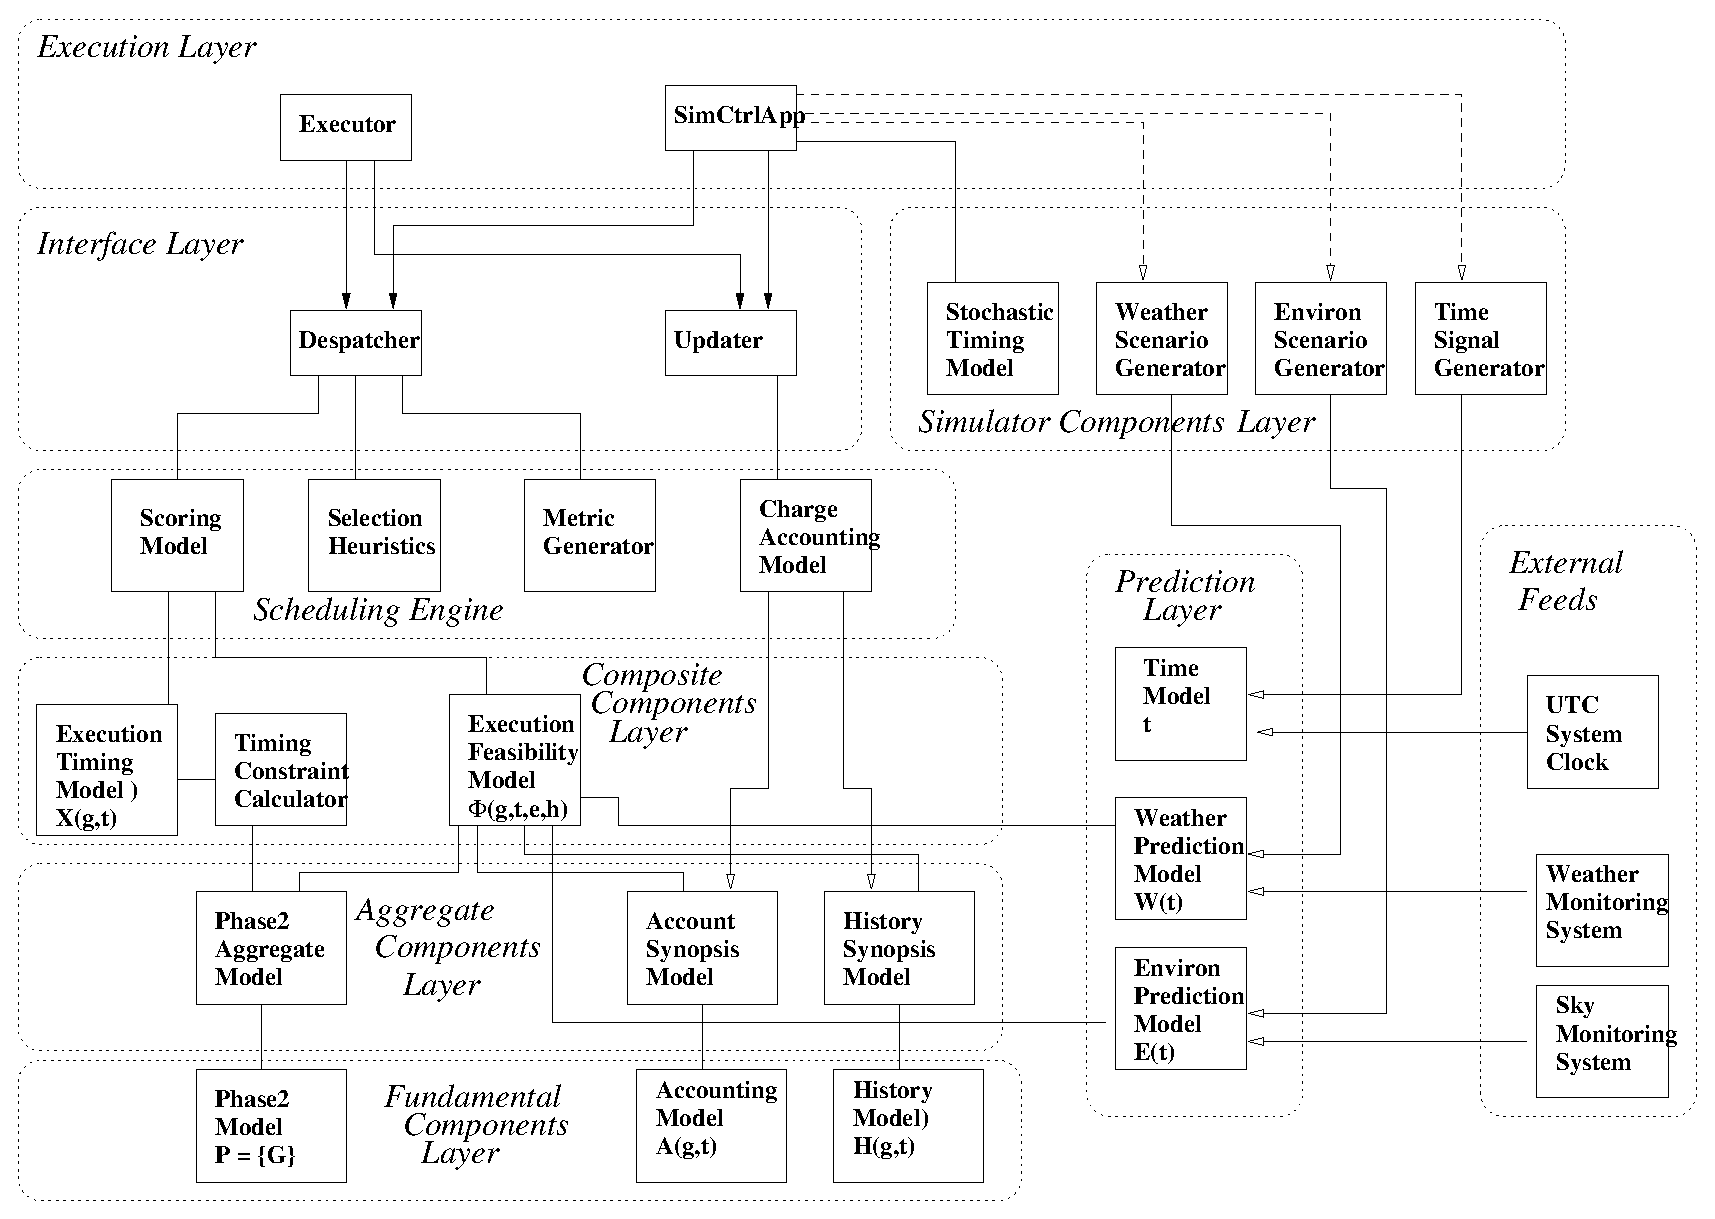
\includegraphics[height=14cm]{figures/sca.eps}
 
      \caption[Scheduling Component Architecture.]
%>>>> use \label inside caption to get Fig. number with \ref{}
      {\label{fig:sca}
      Scheduler Component Architecture consists of a set of fundamental modules and plugin implementations of higher functional modules.}  
   \end{center}
   \end{figure} 
\end{landscape}

\begin{description}
\item[Fundamental Components Layer] contains models which provide access to the Phase II, Accounting and Execution history stored in the ODB.

\item[Aggregate Components Layer] contains models which provide synopses of the models in the Fundamental Components Layer:- \emph{history-synopsis}, \emph{account-synopsis}, \emph{Phase2-aggregation}.

\item[Composite Components Layer] Contains computing models such as the \emph{execution timing model} $X(g,t)$ which provides details of the time required to execute groups by modelling the function of the executor. The \emph{feasibility model} $\Phi(g,t,e,h)$ determines whether a group can be observed under given environmental conditions subject to its observing and timing constraints.

\item[Scheduling Engine Component Layer] Provides \emph{selection heuristics} used to select single groups (or sequences of groups) for execution using the scoring/utility metrics provided by the \emph{scoring model} $S(g,t,e,a,h)$ which determines the gain from performing a specified group. The \emph{cost accounting model} calculates the chargeable cost of performing a group - the time which will be deducted from the proposal's allocation.

\item[Interface Components Layer] Contains the \emph{despatcher}, the executor's entry point for obtaining a schedule and the \emph{updater} which allows the executor to supply observation completion statistics back to the fundamental component models (e.g. to let the history model know that a group was successfully executed).

\item[Executive Components Layer] Represents the external application which requires the services of the scheduler. This will either be the telescope's Robotic Control System, a simulation control application or a user tool.

\item[Prediction Components Layer] Contains models for predicting sky and weather conditions and a \emph{time model} which provides a synchronizing time signal. In an operational situation this is simply the system clock. In a simulated environment it is provided by the simulation controller's time signal generator component.

\item[Simulation Framework Components Layer] Provides \emph{scenario generators} with which to build a simulation environment incoporating time-varying and random effects (weather and sky conditions). A \emph{stochastic timing model} simulates variable execution timing due to uncertainty in mechanical and software processes and provides a time signal to the simulation controller.
\end{description}

%-------------------------------------------
% SHAKEDOWN
%-------------------------------------------
\subsection{Examination of a basic despatch scheduler (BDS) with metric variation}
\label{subsect:bds}
This investigation involved running a series of one-night simulations under different environmental assumptions to see the effect of varying the value of the Heuristic Scoring Metric (HSM) weights used in the scoring model. Specifically a model using just two metrics $f_{OH}$ and $f_{PX}$ were chosen. 
The rational behind this investigation is to provide some initial insight into the usefulness of the various Schedule Quality Metrics (SQM) and to provide a shakedown test of the simulation framework on real data. By selecting 2 seperate but similar nights it should be possible to get a preliminary idea on the range of likely values and variation of SQMs.
Two nights were considered. Both were similar in terms of amount of dark moon time though the actual night lengths were significantly different. Night 1, 13th-14th October 2007 has 75\% lunar dark time out of 12.28 hours night of which 9.52 hours are astronomicaly dark. Night 2, 7th-8th November 2007 has 96.7\% lunar dark time out of 13.03 hours night of which 10.23 hours are astronomicaly dark.
A series of simulations were performed to determine the range of contention statistics for the 2 study nights. Figures \ref{fig:cont4_ensemble} and \ref{fig:cont6_ensemble} show ensemble results from a large number of simulations for the 2 nights.

\begin{figure}[h]
 \begin{center}
    \includegraphics[scale=0.5, angle=-90]{figures/cont4_ensemble.eps}
    \caption{Contention profile ensembles for case study night 1} 
  \label{fig:cont4_ensemble}
 \end{center}
\end{figure}

\begin{figure}[h]
 \begin{center}
    \includegraphics[scale=0.5, angle=-90]{figures/cont6_ensemble.eps}
    \caption{Contention profile ensembles for case study night 2} 
  \label{fig:cont6_ensemble}
 \end{center}
\end{figure}


For both nights simulations were run using a basic rank scoring selection mechanism $\mathcal{S}_{BEST}$ which selects the highest scoring group from the set of candidate metrics. In addition a second simulation was performed using a random selection model $\mathcal{S}_{Random}$ in which all candidates have equal chance of selection irrespective of their relative scores. This was to provide an indication of how well the normal selection and scoring mechanisms perform against a baseline.

A major conclusion of this investigation was that the objective function (scoring heuristic) with the highest weighting copletely dominates the final scoring - it is feasible to trade off only a small number of independant objectives. Any low weighted functions effectively contribute random noise to the system. This is mainly due to the fairly evenly distributed values of the variables which the metrics measure.

% the dominant weighted function determines final scoring and it is feasible only to trade off a small number of independant objective functions. 

%If its not selected for it wont come out in the SQMs.

%Add a histogram of a-rank to show scoring noise effect.

%-------------------------------------------
% MAM
%-------------------------------------------
\subsection{Man against machine}
\label{subsect:mam}
In this experiment an experienced human scheduler is pitted against a series of automated schedulers to see who can achieve the \emph{best} (highest value) schedule.
%description - likely problems assumptions errors how handled, input forms, what they did - notes from subject, how measured, results-comparison with other schedulers.

Selecting appropriate groups to perform is a complex task. There are many trade-offs to be made between the various competing preferences and constraints. When the schedule is heavily loaded, i.e. there are potentially more observations to perform than could be accomodated even under ideal conditions, the job of the scheduler becomes extremely difficult. A major problem is to determine just what those tradeoffs are - i.e. just how much more important is a high priority, non-urgent group relative to a medium priority urgent group?. It is because it is difficult to quantify these relative weights that we turn to the human scheduler. A human makes these sort of trade-offs on a daily basis - often with little knowledge they are doing it - if we set a human up to perform the task we might be able to deduce from what they have done and the choices they have made some of the rules they are using (often without realizing) and the relative weighting they employ. Additionally it was thought that it would be useful just to know if a human was in fact capable of \emph{beating} an automated scheduler in terms of the standard SQMs. To date, data has been obtained from the human scheduler and a baseline simulation has been run for comparision. The results of these are awaiting detailed analysis.

%-------------------------------------------
% LTS
%-------------------------------------------
\subsection{Long period study}
\label{subsect:lts}
This study was aimed at comparing the effectiveness of different scheduling algorithms and configurations under varying conditions over an extended period. In particular the effectiveness of schedulers under varying load and environmental stability. In order to make these comparisons it is neccessary to develop generators to create phase2 models with specific load characteristics and environmental models with specific stability criteria in order to have independant variables to measure performance against.

\subsubsection{Environment Models}
From section~\ref{subsect:ecs} we see that the environmental conditions at the telescope site (specifically seeing) are seen to vary over different timescales from minutes to hours. The seeing conditions are split into several bands defined as: (G) good ($s < 0.8''$), (A) average ($0.8'' < s <= 1.3''$), (P) poor ($1.3'' < s <= 3.0''$) , (U) usable ($3'' < s <= 5''$), (B) bad/unusable ($s > 5''$). From the point of view of scheduling it is only these bands which matter. So long as the seeing varies within any band, neither contention or scoring of groups are affected. When the seeing transitions between bands both are affected. 

From a defined set of environment model parameters we can generate any number of scenarios (effectively instantiations of the model) - it would be useful to see if we get variation in results and indeed in the SQMs from different scenarios generated by the same model - if this variation is large we will have to run many more simulations and there will be x-errors in addition to the expected y-errors.

Seeing variation can be modelled by a simple transition matrix $P(t)$ where each element $P_{ij}(t)$ represents the cumulative probability of transitioning from state i to state j within a period t. The diagonal elements $P_{ii}(t)$ represent the probability of \emph{remaining} in a particular state for time upto t. 
\begin{equation}
 \left( 
\begin{array}{ccccc}
  P_{gg}(t) & P_{ga}(t) & P_{gp}(t) & P_{gu}(t) & P_{gb}(t)\\
  P_{ag}(t) & P_{aa}(t) & P_{ap}(t) & P_{au}(t) & P_{ab}(t)\\
  P_{pg}(t) & P_{pa}(t) & P_{pp}(t) & P_{gu}(t) & P_{pb}(t)\\
  P_{ug}(t) & P_{ua}(t) & P_{up}(t) & P_{uu}(t) & P_{ub}(t)\\
  P_{bg}(t) & P_{ba}(t) & P_{bp}(t) & P_{bu}(t) & P_{bb}(t)

\end{array} 
\right)
\end{equation}

 The relative distribution of time spent in each band is of little interest from the point of view of these studies - only the stability or frequency of change is important.  The diagonal elements were therefore set to the same value based on a stability parameter $\tau_E$ such that the probability of remaining in a given band/state for upto time t is given by $P_{ii}(t) = 1 - \exp{t/\tau_E}$. The Bad and usable bands are also of less interest - bad indicates no observing possible, and in practice relatively few groups are ever setup with such lax seeing constraints, consequently the array is reduced to 3x3. The non-diagonal elements are each set to the same value, namely $P_{ij} = 0.5*(1 - P_{ii})$. 


A specific seeing scenario is generated by taking random intervals calculated from $-\tau_E \ln{(1-R)}$ where R is a random number in $[0,1]$. At each period the seeing is allowed to change randomly to another value (band) - we are not particularly interested as to which band it change or how the time spent in the different bands is distributed, only how frequently it is changing.

\subsubsection{Generated Phase II model characterisation}
Before embarking on any scheduler comparisions there is a need to decide which type of Phase II model to use. A real model suffers from the ODB evolution problem. From  Fig.~\ref{fig:c60_odb_av} which shows the variation of average nightly contention $C_C$ for a snapshot taken on the first night, we see the contention declines over a period. This is due to the pattern in which observations are entered into the system. A sizeable number of observations are \emph{short-term} and only entered into the ODB a day or so before they are required. In some cases - particularly where automated agents are involved, the observations may be entered minutes before they become activated. This information cannot be captured by a snapshot of the ODB at a given time and so the observed quality and characterisation measures drift away from what would be observed if the ODB model were being regularly replenished.

\begin{figure}[h]
\begin{center}
   \includegraphics[scale=0.5, angle=-90]{figures/c60_odb_cav.eps}
  \caption{Variation of average contention $\bar{C_c}$ from ODB snapshot}
 \label{fig:c60_odb_av}
 \end{center}
\end{figure}

 With a generated model however, group activations can be spread out over a specified period (say several months) so new groups are appearing in the schedule every day - like the real ODB but in that case they are typically not entered until just before required so using daily snapshots, we do not know about them in advance and cannot take them into account easily.
   
Additionally, it would be useful to see if different schedulers perform better than others when faced with phase2 models (pools of observation requests) with different \emph{weight} or \emph{load} characteristics.  i.e. is one scheduler better at handling \emph{light} loading and another better at handling \emph{heavy} loading.

A Phase2 Model generator was designed to create phase2 models with varying characteristics. This generator has a large number of configurable parameters. 


From a given generator model (e.g. $P_l$) we can generate any number of actual instances - ideally these would all have the same measurable characteristics (e.g. $\bar{C_c}$) but this is not guaranteed. Tests were run using each of the generator models in order to determine the variation of characteristics. The measurable characteristic chosen was $\bar{C_{dc}}$ - the average dynamic contention over the measurment period. A simple scheduler was chosen using best-score selection and a single $f_{OH}$ metric - i.e. the target which was highest relative to maximum attainable elevation was chosen at each sweep. We are not interested in the scheduler here, only the variability of the generated  P2 characteristics. Simulations were run for the middle 30 days of the generated models and the values of $\bar{Q_{SU}}$ and $\bar{Q_{XT}}$ are plotted against $\bar{C_c}$ for each model. The results are shown in Fig.~\ref{fig:p2_gen_su} and  Fig.~\ref{fig:p2_gen_xt}.

\begin{figure}[h]
\begin{center}
 \includegraphics[scale=0.5, angle=-90]{figures/p2_gen_qsu.eps}
 \caption[Variation of $Q_{SU}$ with $C_C$ for variable phase2 generator models.] 
   {Variation of $Q_{SU}$ with $C_c$. Each point represents a single phase 2 model generated by one of 4 initial sets of generators.}
\label{fig:p2_gen_su}
\end{center}
\end{figure}


\begin{figure}[h]

\begin{center}
 \includegraphics[scale=0.5, angle=-90]{figures/p2_gen_qxt.eps}
 \caption[Variation of $Q_{XT}$ with $C_C$ for variable phase2 generator models.] 
   {Variation of $Q_{XT}$ with $C_c$. Each point represents a single phase 2 model generated by one of 4 initial sets of generators.}
\label{fig:p2_gen_xt}
\end{center} 
\end{figure}

\subsubsection{Basic Despatch Scheduler}
The basic despatch scheduler (BDS) uses a weighted metric scoring model and best ranked selection heuristic. All candidate groups are scored and ranked, the \emph{best} candidate at the instant being selected without reference to any future potential. 


\subsubsection{Look-Ahead Schedulers}
Look-ahead schedulers work on the assumption that the environmental (and weather) conditions will remain stable for a given period of time (the parameter $\Delta E$ in an environment scenario represents the length of this stable period). By suitable selection of the length of look-ahead horizon it is hoped that a better degree of optimization can be achieved than by a BDS. Identification of the size of this horizon is clearly important. Choosing a value too large means that the schedule generated is likely to break (reducing the optimizing effect). Selection of too short a horizon wastes potential optimization opportunities. 

\subsubsection{Quantum Look-Ahead Scheduler} QLAS is an implementation of a look-ahead scheduler in which lists of potential candidates are generated at fixed intervals $\Delta \tau _q$ for upto a given horizon length $H$ in the future. A number of sequences $N_s$ are generated at random from these candidate lists and evaluated. The \emph{best} (highest value) sequence is selected and then executed until it either completes or breaks e.g. due to changing environmental conditions.
\begin{figure}[htp]
\begin{center} 
  \includegraphics[scale=0.5, angle=-90]{figures/qsa3_su.eps}
  \caption[Effect of horizon length on $Q_{SU}$ metric under unstable environment $\Delta E = 0.5h$]
{\label{fig:suplot} Effect of horizon length on $Q_{SU}$  metric under unstable environment $\Delta E = 0.5$ hours. BDS exceeds all QLAS horizons during second half but QLAS performs marginally better in earlier half of scenario.}
\end{center}
\end{figure}

\subsubsection{Experimental setup}
The two schedulers already discussed (BDS and QLAS) were compared under varying environmental scenarios. Seperate tests were performed to determine the effects of varying the look-ahead horizon $H$ and sequence count $N_s$.
The same scoring model was used for both BDS and QLAS. Single environmental scenarios were used based on environmental stability parameter $\Delta E$ ranging from  0.5 to 4 hours. The Phase II model (MD1) was used. This produces a \emph{medium} load and has a high percentage of observations requiring \emph{dark moon} conditions resulting in pronounced monthly variations in most quality metrics (see dips around $20^{th}$ May and $18^{th}$ June in Fig.~\ref{fig:suplot}). The stochastic execution timing model was swapped for a fixed timing model. Statistical variation is thus not well handled due to lack of time available to run simulations so no error bars are shown.

\subsubsection{Initial comparison}
 An initial test was made using a highly unstable environment ($\Delta E = 0.5$ hours). Fig.~\ref{fig:suplot} shows the results of a series of runs using BDS and QLAS with $H$ values of 0.5, 1 and 2 hours. As can be seen under these (severe) conditions BDS is as or more effective then QLAS. It was also found that BDS performs consistently better at filling the available time. 

\subsubsection{Comparison of effect of varying horizon $H$}
A set of horizon lengths ranging from 0.5 to 4 hours were tested yielding the results displayed in Fig.~\ref{fig:hor_denv}. As can be seen, increasing $H$ yields some overall improvement over the BDS though clearly this is not constant, i.e. some of the time BDS beats all QLAS examples, especially at lower $\Delta E$ as might be expected. Study of the amount of available execution time actually used shows somewhat unexpectedly that QLAS tends to be less efficient overall than BDS - this is accounted for by the fact that BDS always tries to select something to do, QLAS will sit idle for short periods in order to await a more lucrative observation. There are clearly some dangers in this approach, especially if the conditions should change during the wait thus leaving the awaited high-value observation no longer available, this then becomes wasted time. 



\subsubsection{Comparison of effect of changing sequence count $N_s$} 
In order to examine the effect of varying the sequence count in QLAS, a series of simulations were run with $N_s$ varying from 10 through to 10000 in logarithmic progression and with fixed values of $H = 1$ hour and $\Delta \tau _q = 60$ secs. The experiments were performed under 3 different environmental scenarios with $\Delta E$ selected at 1,2 and 4 hours along with a baseline comparison performed using BDS. The results are given in Fig.~\ref{fig:ns_denv} and show that the schedule quality improves significantly as we move to higher $N_s$ values though with diminishing effect. At low $N_s$ BDS always beats QLAS. These results are more or less as expected. The QLAS is looking for the best sequence from a potentially very large number of possible sequences. With small $N_s$ it stands a good chance of missing  the highest scoring sequences. As $N_s$ increases we are searching more of the space of possible solutions. 

%% FIG 2
\begin{figure}[htp]
\begin{center}
  \includegraphics[scale=0.5, angle=-90]{horiz_env_su.eps}
\caption[Effect of look-ahead horizon length $H$ on $Q_{SU}$ under a range of environmental conditions]
{\label{fig:hor_denv}Effect of look-ahead horizon length $H$ on $Q_{SU}$  metric under a range of environment model stability parameter $\Delta E$ ranging from 0.25 to 4 hours. BDS provides fairly stable baseline with average $Q_{SU}=74.09$. QLAS shows reduced effectiveness (lower $Q_{SU}$) under unstable conditions (low $\Delta E$) for all tested horizon lengths. As environment becomes more stable ($\Delta E$ increasing) the longer horizon QLAS becomes increasingly more effective - i.e. the optimization effect.}
\end{center}
\end{figure}

%% FIG 3
\begin{figure}[htp]
\begin{center}
  \includegraphics[scale=0.5, angle=-90]{ns_env_su.eps}
\caption[Effect of sequence count $N_s$ on $Q_{SU}$ under a range of environmental conditions]
{ \label{fig:ns_denv}Effect of sequence count $N_s$ on $Q_{SU}$ under a range of environment model stability parameter $\Delta E$. $Q_{SU}$ is seen to increase with $N_s$ in line with expectation as more of the search space of potential solutions is explored but with diminishing effect at high $N_s$.}
\end{center}
\end{figure}

%-------------------------------------------
% TBD
%-------------------------------------------
\newpage
\section{Conclusions}
It has proved difficult to devise any Schedule Quality Metric (SQM) which is genuinely independant of the Heuristic Scoring Metrics used to generate schedules in this domain consequently most of the SQMs employed relate directly to those objective functions. The operating environment of the telescope is well characterized - though there is a wealth of archive data available our own high cadence data extends only over a short period (around 5 years now) and is insufficient to derive any long term trends or to provide statistically meaningful results. Nonetheless the prediction scheme tested does provide reasonably good results. 

A great deal of insight has been gained into the range of architectural components required to build observation scheduling engines. It has proved quite straightforward then to actually build engines from these. The development of a simulation framework brought out some unexpected requirements -such as the need to provide a stochastic model for the execution timing of observations. Constructing simulation controllers (for specific experiments) brought out requirements for a number of additional components e.g. synchronization of simulation time between the simulation controller and the running scheduler due to the finite (real) time taken by the scheduler while the simulator ran at vastly accelerate rate. 

Experiments using the Basic Despatch Scheduler and comparison of the effects of varying the weightings of the objective scoring functions revealed that the final schedule quality is heavily dependant on the weighting used. Due to the generally even distribution of each of the scheduling variables only the highest weighted variable has much effect on the final selection so that the other variables act more like random noise. It was found that adding some bias to the selection heuristic improved the overall quality but produced more variation between individual schedule runs. 

Comparison of the despatch and look-ahead schedulers has so far revealed that the look-ahead scheduler performs better under stable conditions but that the despatcher is more effective when conditions are changing rapidly. The length of the look-ahead horizon for optimal scoring is related to the characteristic time of the environmental stability measure.


\newpage
\section{Work Plan}

With reference to Fig.(\ref{fig:powgantt}), the work to M.Phil was completed by mid 2008. Much of the work to extend to Ph.D has been completed and some additional simulations and analysis of data already collected remains.
\subsection{Work to M.Phil}
\begin{itemize}
\item \emph{Literature review}.
\item \emph{Preliminary architecture design}.
\item \emph{Analysis of environmental data from LT archive and embedded instrumentation}.
\item \emph{Design and implement basic on-demand despatch scheduler}.
\item \emph{Test scheduler}.
\item \emph{Design, implement and test simulation framework}.
\item \emph{Develop problem complexity and schedule quality metrics}.
\item \emph{Run simulations using despatch scheduler and framework}. 
\item \emph{Analysis simulation results}.
\end{itemize}

\subsection{Additonal work to Ph.D (already completed)}

\begin{itemize}
\item \emph{Design and implement look-ahead scheduler (LAS)}.
\item \emph{Run basic simulations using LAS}. 
\item \emph{Enhance simulation framework with environment and weather scenarios}. 
\end{itemize}

\subsection{Additonal work to Ph.D (remaining to complete)}

\begin{itemize}
\item \emph{Run simulations using LAS under enhanced framework}. Much of this has been completed but further work is required to investigate the effects of Phase II volatility - the manner in which the database content varies from day to day and over the course of the semester. This will be particularly important where the users have access to the database to enter their own observations in real-time and where external software agents are inserting new observations.
\item \emph{Analysis of simulation results}. This work has been started (section~\ref{subsect:lts}) but more detailed analysis remains to be done on the collected data.
\end{itemize}

%\item Data from the \emph{Man against Machine Study}(section~\ref{subsect:mam}) has been analysed for the human part of the experiment but simulations for the machine part remain to be performed and comparisons made.

%%%%%\clearpage
\begin{landscape}
   \begin{figure}[htp]
   \begin{center}
      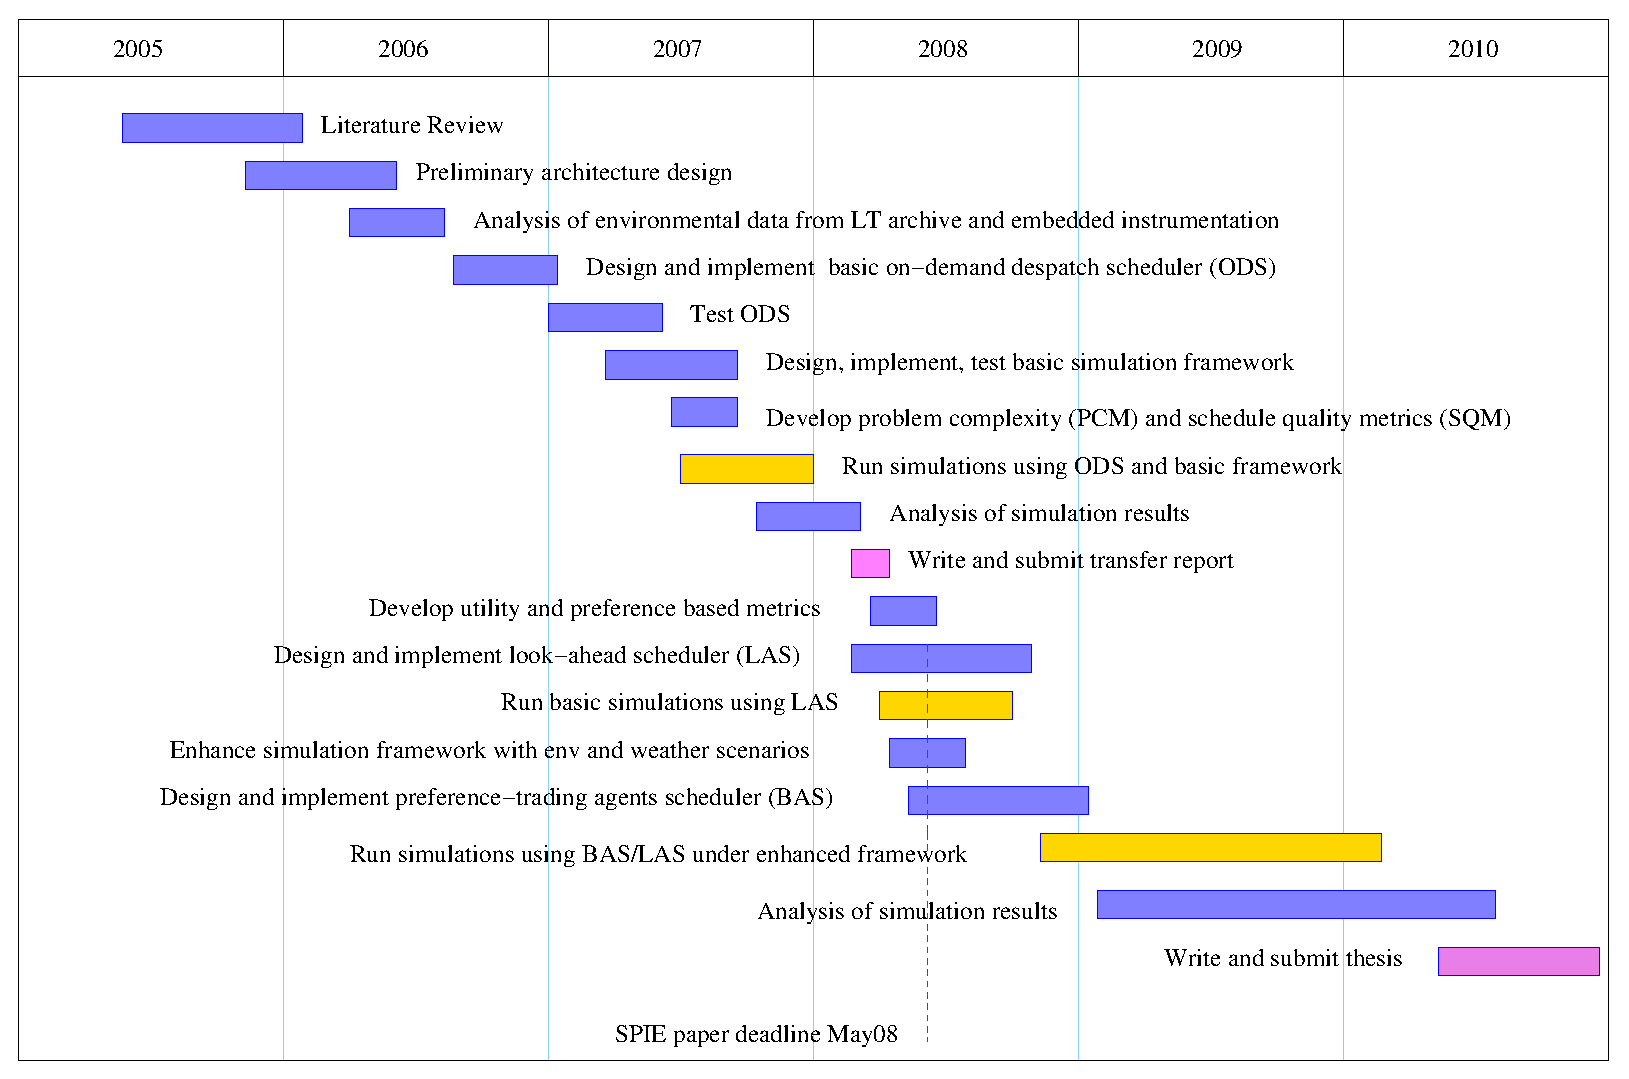
\includegraphics[height=14cm]{figures/gantt.eps}
 
      \caption[Work plan.]
%>>>> use \label inside caption to get Fig. number with \ref{}
      {\label{fig:powgantt}
      Plan of work.}  
   \end{center}
   \end{figure} 
\end{landscape}

\newpage
\bibliography{biblio}
\bibliographystyle{apalike}

\end{document}
